\section{El modelo Transformer}

A finales del año 2017 se presentó un nuevo modelo que vino a revolucionar el área de Procesamiento
de Lenguaje Natural, El Transformer \cite{Vaswani}. Una de sus principales características es la
capacidad de procesar la información de alguna secuencia de forma paralela, caso contrario a las
Redes Neuronales Recurrentes, donde la información se procesa recurrentemente. Gracias a ello,
la capacidad de \textit{recuerdo} no se ve afectado por el problema de \textit{El desvanecimiento
del Gradiente} específicamente cuando el problema es trabajar con secuencias  bastante largas.

\textit{El Transformer} puede ser visto como otro modelo \textit{seq2seq} (Secuencia a Secuencia)
\ref{fig:trans_seq2sqe}, formado en por dos etapas, la primera encargada de codificar la información de entrada
y la segunda de decodificarla, pero la su principal característica es que aplica el mecanismos de
\textit{Self-Attention} para capturar las dependencias globales entre la entrada y la salida. Dada
una secuencia de entrada $X = (x_1, x_2, \dots, x_n )$ con $n$ como el tamaño de la secuencia,
el codificador produce una representación intermedia
$Z = (z_1, z_2, \dots, z_n)$ al igual que los modelos \textit{seq2seq}. El decodificador usa la
secuencia $Z$ para generar la secuencia de salida
$Y = (y_1, y_2, \dots, y_m)$ uno a la vez (en modo inferencia), con $m$ como el tamaño de la
secuencia de salida. Nótese, que el generar una salida a la vez el decodificador tiene que ser auto-regresivo.
Usa la salida anterior $y_{i-1}$ como entrada adicional para generar la siguiente salida $y_i$. Por
ello, durante entrenamiento el modelo es alimentado con entradas y salidas desfasadas en un tiempo.

\begin{figure}[ht!]
    \centering
    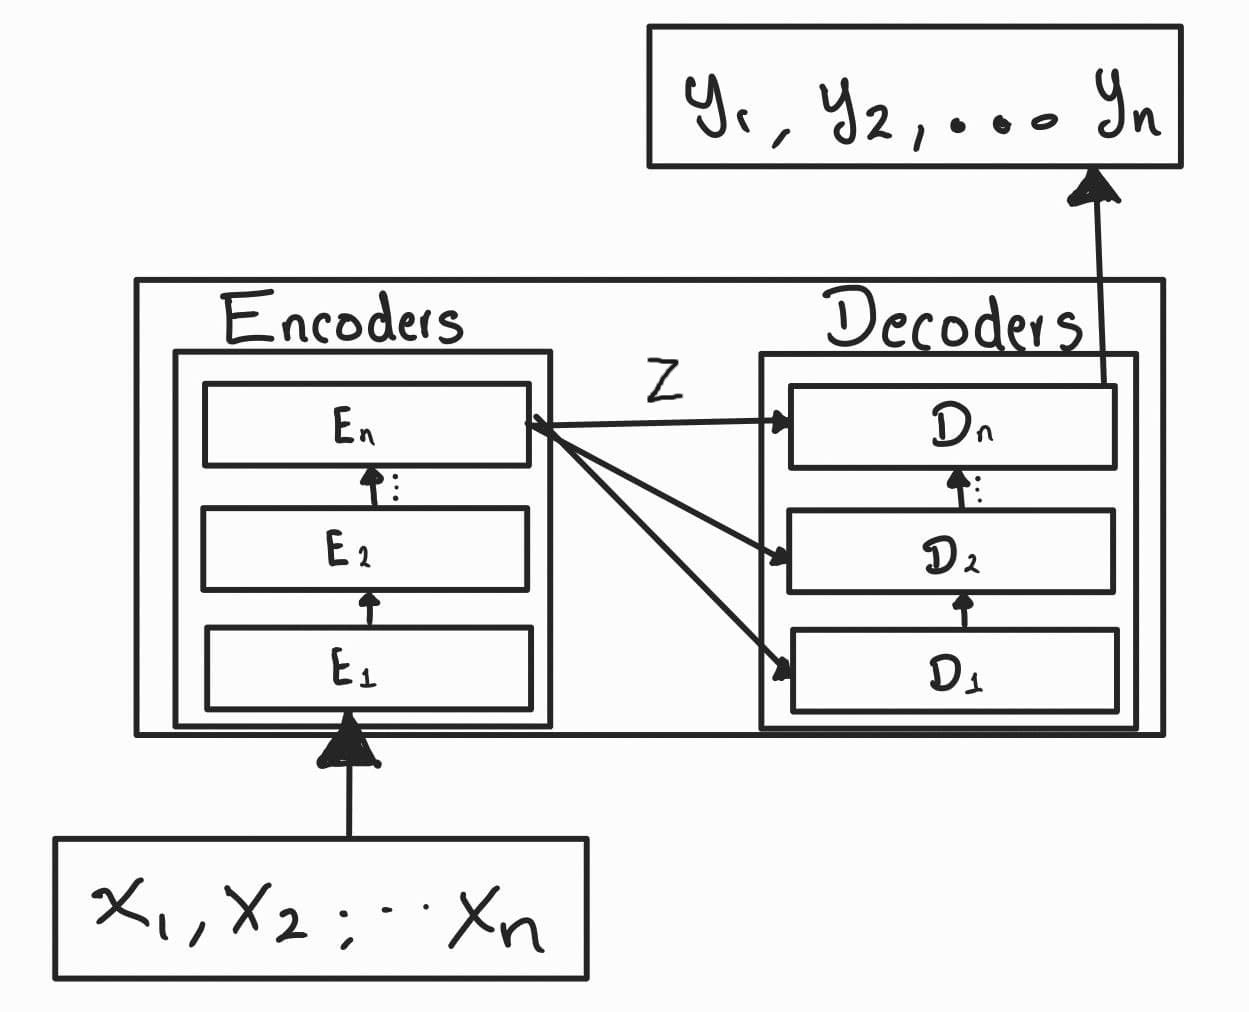
\includegraphics[width=0.4 \textwidth]{Chapters/1. Transformer/Figures/transformer/t_seq2seq.jpg}
    \caption{Modelo Transformer generalizado como modelo Secuencia a Secuencia}
    \label{fig:trans_seq2sqe}
\end{figure}

Poner ejemplo de Transformer en con la figura de arriba en tiempo de entrenamiento e inferencia aquí.

\subsection{El Codificador y Decodificador}

El \textit{Modelo Transformer} está formado por multiples codificadores  y decodificadores apilados e inter-conectados,
Como observamos en la figura \ref{fig:trans_seq2sqe}. El codificador consta de dos partes,
la primera de ellas aplica \textit{Self-Attention} múltiples veces sobre la misma entrada
(\textit{Multi-HeadSelf Attention}) y la segunda capa representada solo por una red
\textit{Feed-Forward} cuya entrada es la salida de la capa anterior.
Véase la figura \ref{fig:trans_encoder}.


\begin{figure}[ht!]
\centering
    \begin{minipage}{.4\textwidth}
        \centering
        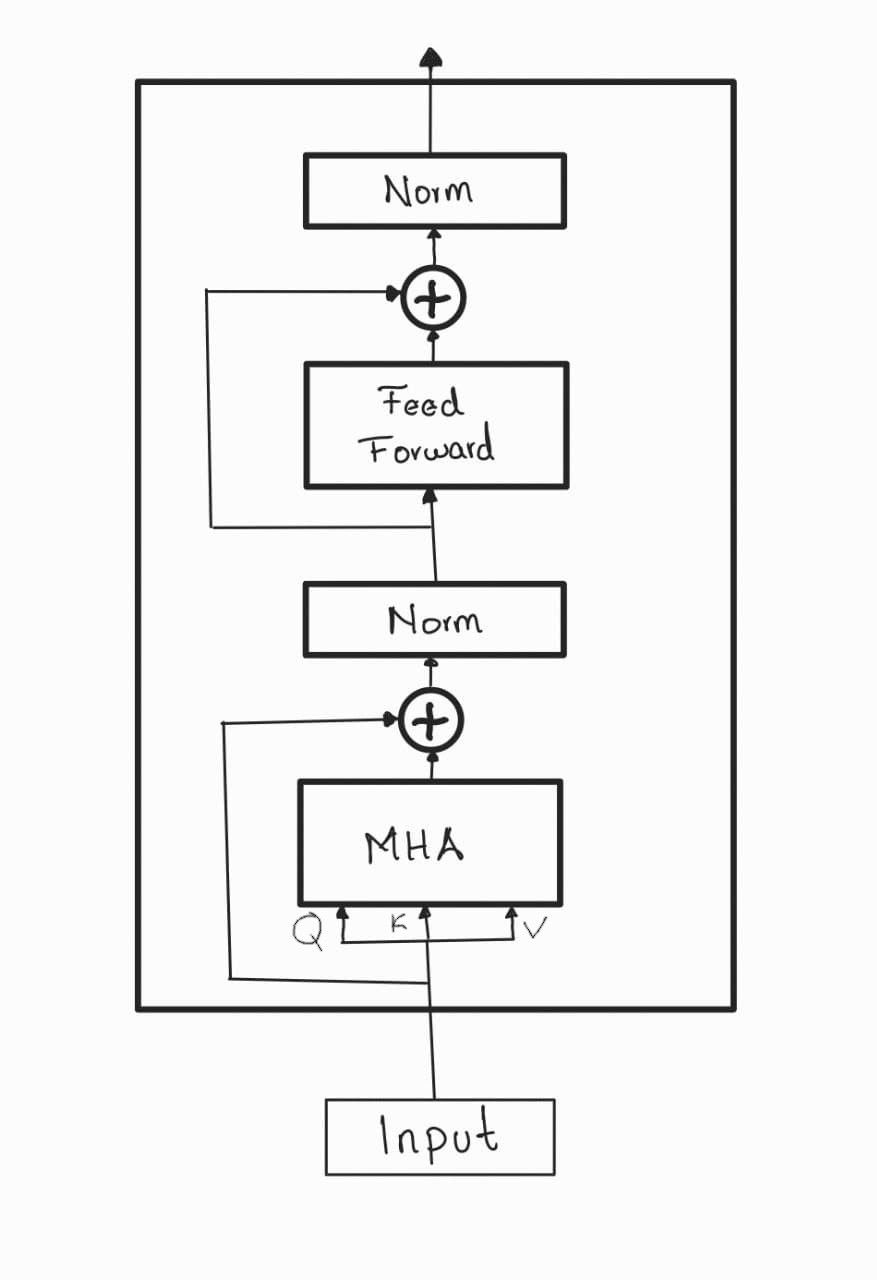
\includegraphics[width=0.7 \textwidth]{Chapters/1. Transformer/Figures/transformer/encoder.jpg}
    \end{minipage}
    \begin{minipage}{.5\textwidth}
        \begin{equation*}
            \begin{split}
                mha = MHA(X, X, X)\\
                norm = Norm( mha + X)\\
                f = FeedForward(norm)\\
                Encoder(X) = Norm(f + norm)
            \end{split}
            \label{eq:trans_enc}
        \end{equation*}
    \end{minipage}
    \caption{Etapa Codificadora del Modelo Transformer. Pseudocódigo}
    \label{fig:trans_encoder}
\end{figure}


El decodificador tiene una estructura similar al codificador con una etapa adicional intermedia
de \textit{Multi-Head Attention} aplicada sobre la salida de la pila de codificadores. También, la
primer capa de atención sufre un ligero cambio un su forma de operación, necesitando enmáscarar (al
momento en que se realiza el entrenamiento) la atención prestada del pasado al futuro. Esto es
debido a que el decodificador se encarga de generar una secuencia (en modo inferencia) uno a la vez
usando solamente la salida anterior y por tanto no tiene conocimiento de salidas futuras.

\begin{figure}[ht!]
\centering
    \begin{minipage}{.4\textwidth}
        \centering
        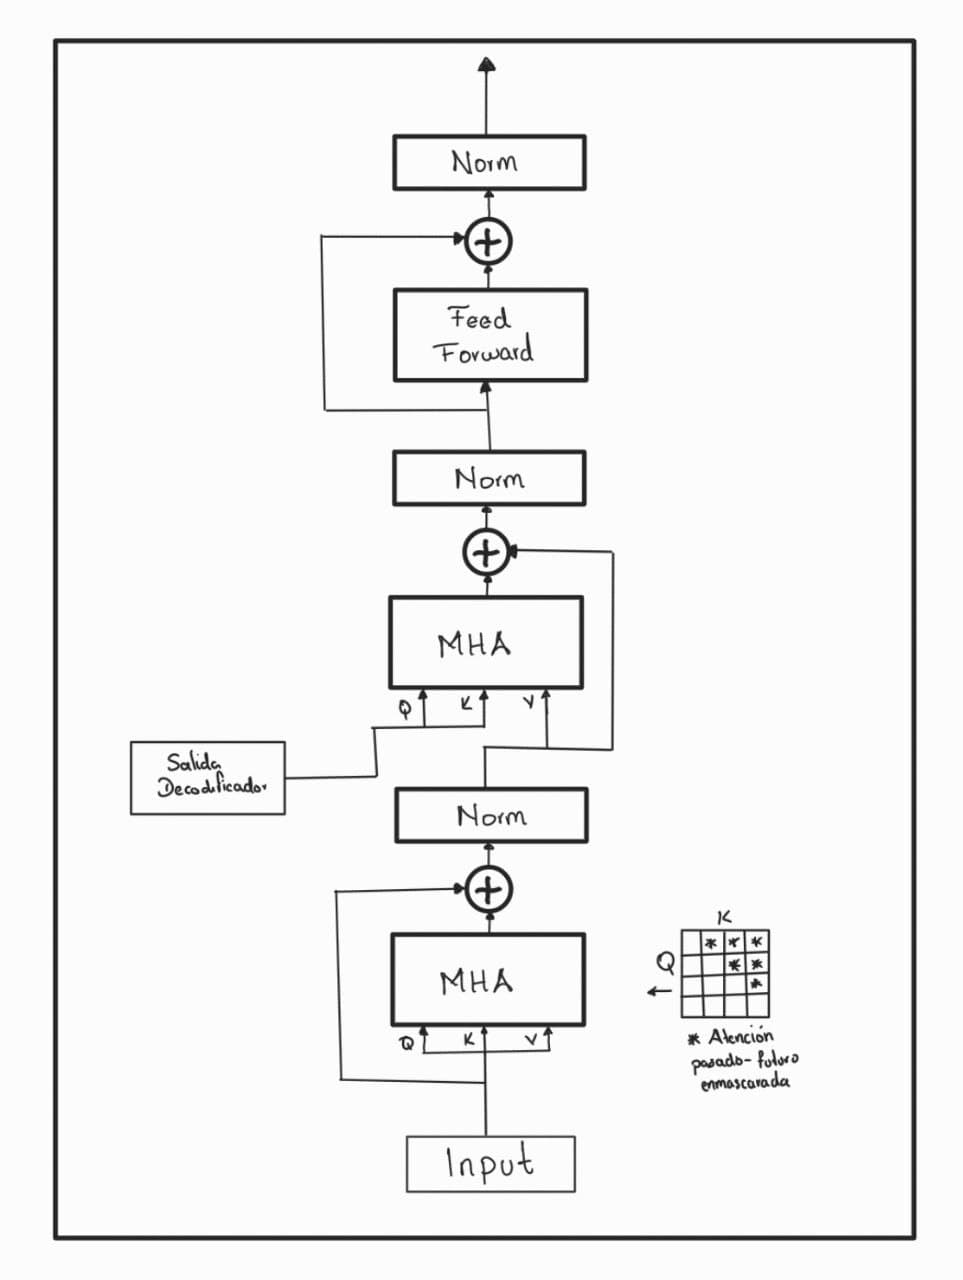
\includegraphics[width=1.0 \textwidth]{Chapters/1. Transformer/Figures/transformer/decoder.jpg}
    \end{minipage}
    \begin{minipage}{.5\textwidth}
        \begin{equation*}
            \begin{split}
                mha_1 = MHA(X, X, X)\\
                norm_1 = Norm( mha_1 + X)\\
                mha_2 = MHA(enc_{out}, enc_{out}, norm_1)\\
                norm_2 = Norm( mha_2 + X)\\
                f = FeedForward(norm_2)\\
                decoder(X) = Norm(f + norm_2)
            \end{split}
            \label{eq:trans_dec}
        \end{equation*}
    \end{minipage}
    \caption{Etapa Decodificadora del Modelo Transformer. Pseudocódigo}
    \label{fig:trans_decoder}
\end{figure}

\subsection{Multi-Head Self-Attention}

En la sección \ref{section:att} se detalla una generalización de la atención y diversas variantes usadas
a lo largo de la literatura. El modelo original que introdujo a los Transformers usa en especial la variante
\textit{Scaled Dot-Product Attention}\cite{Vaswani}:

\begin{equation}
    Attention(q, k, v) = softmax(\frac{q k^\top}{\sqrt{d_k}}) v
    \label{eq:trans_att_gen}
\end{equation}

El Transformer está basado en la idea de de aplicar atención multiples veces, al usar varias cabezas
de atención, Multihead-Self-Attention (MHA), permite  al modelo conjuntamente atender a información
en diferentes posiciones desde diferentes subespacios de representación. Finalmente todas las cabezas
de atención son concatenadas y resumidas pasándolos las dimensiones del espacio original de las
entradas \ref{eq:mha}

\begin{equation}
    mha(Q, K, V) = Concat(head_1,head_2,head_3,..., head_h)W^O
    \label{eq:mha}
\end{equation}

$Q, K \in \mathbb{R}^{n \times d_{k}}$ y $V \in \mathbb{R}^{n \times d_{v}}$ son los embeddings de
entrada a cada capa de atención del codificador y decodificador como se observa en las figuras,
\ref{fig:trans_encoder} \ref{fig:trans_decoder}, $n$ es el tamaño de la
secuencia, $d_k$ y $d_v$ son los tamaño del embedding y $h$ el número de cabezas de atención. Cada cabeza es


En el caso transformer, tenemos un conjunto embeddings sobre las cuales se aplica atención. Si bien
no representan necesariamente las consultas, llaves, y valores necesarios para la attention generalizada,
podemos obtener estas representaciones transportándo a sus espacios respectivos a través de alguna
transformación aprendida conjuntamente con el entrenamiento del modelo.

Para un conjunto de
Embeddings o representaciones $E_Q \in \mathbb{R}^{n \times d_k}$,
$E_K \in \mathbb{R}^{n \times d_k}$ y $E_V in \mathbb{R}^{n \times d_v}$ donde $n$ es el número
embeddings, $d_k$ y $d_v$ son las dimensiones de cada uno, la atención se calcula como:

\begin{equation}
    Attention(E_QW_i^Q, E_KW_i^K, E_VW_i^V) = softmax\Big(\frac{QW_i^Q (KW_i^K)^T}{\sqrt{d_k}}\Big) VW_i^V
    \label{eq:trans_att}
\end{equation}

el término de escalamiento $\sqrt{d_k}$ ayuda a evitar que la magnitud de los productos puntos calculados
entre cada consulta y llave crezcan demasiado, y la función $softmax$ puede ser más estable al evitar
regiones donde los gradientes son muy pequeños\cite{Vaswani}.
